\chapter{Dynamisches Programmieren}
Dynamische Programmierung ist eine Methode zum algorithmischen Lösen von Optimierungsproblemen.
Es kann dann erfolgreich eingesetzt werden, wenn das Optimierungsproblem aus vielen gleichartigen Teilproblemen besteht,
und eine optimale Lösung des Problems sich aus optimalen Lösungen der Teilprobleme zusammensetzt.
In der dynamischen Programmierung werden zuerst die optimalen Lösungen der kleinsten Teilprobleme direkt berechnet und dann geeignet zu einer Lösung eines nächstgrößeren Teilproblems zusammengesetzt.
Dieses Verfahren setzt man fort, bis das ursprüngliche Problem gelöst wurde.
Einmal berechnete Teilergebnisse werden in einer Tabelle gespeichert.
Bei nachfolgenden Berechnungen gleichartiger Teilprobleme wird auf diese Zwischenlösungen zurückgegriffen, anstatt sie jedes Mal neu zu berechnen.
Wird die dynamische Programmierung konsequent eingesetzt, vermeidet sie kostspielige Rekursionen, weil bekannte Teilergebnisse wiederverwendet werden.
Die Laufzeit eines dynamischen Programmieralgorithmuses ist Tabellengröße \(\cdot\) Aufwand pro Eintrag.

\subsubsection{Beispiel}
Ein Läufer nimmt in jeden Schritt 1 oder 2 Stufen auf einmal.
Wieviele Möglichkeiten gibt es, \(n\) Stufen herrauf zu steigen?
\begin{eqnarray*}
t_{1} &=& 1\\
t_{2} &=& 2\\
t_{n} &=& t_{n-1} + t_{n-2}
\end{eqnarray*}
Man kann zeigen das \(t_{n} \in \mathcal{O}(1,618^{n})\) liegt.
Wenn \(t_{n}\) rekursiv berechnet wird, werden die meisten \(t_{n}\) mehrfach berechnet, siehe Abbildung \ref{fig:ProgLaufer}.
Um \(t_{n}\) durch dynamische Programmierung zu berechnen, speichert man die Werte von \(t_{n}\) in einem Feld.
Die Laufzeit beträgt somit: \(\mathcal{O}(n)\cdot\mathcal{O}(1) = \mathcal{O}(n)\).
\newpage
\begin{figure}[htbp]
	\begin{center}
		\begin{tikzpicture}
		\Tree [
			.\(t_{n}\)
			[.\(t_{n-1}\)
				[.\(t_{n-2}\) ]
				[.\(t_{n-3}\) ]
			]
			[.\(t_{n-2}\)
				[.\(t_{n-3}\) ]
				[.\(t_{n-4}\) ]
			]
		]
		\end{tikzpicture}
	\end{center}
	\caption{Verdeutlichung der mehrfachen Berechnung von Werten}
	\label{fig:ProgLaufer}
\end{figure}
\begin{figure}[htbp]
\begin{lstlisting}[language=java, caption={Beispielimplementierung in Java}]
for(i=1; i<=n; i++) {
	if(n==1)
		t[n] = 1;
	else if(n==2)
		t[n] = 2;
	else
		t[n] = t[n-1] + t[n-2];
}
\end{lstlisting}
\end{figure}

\section{Editierdistanz}
Die Editierdistanz zwischen zwei Zeichenketten ist die minimale Anzahl von Einfüge-, Lösch- und Ersetz-Operationen, um die erste Zeichenkette in die zweite umzuwandeln.
In der Praxis wird die Editierdistanz zur Bestimmung der Ähnlichkeit von Zeichenketten beispielsweise zur Rechtschreibprüfung, DNA-Sequenzvergleich oder bei der Duplikaterkennung angewandt.

Gegeben seien zwei Strings a, b, wieviele Editieroperationen sind nötig, um a in b zu überführen?
\begin{figure}[htbp]
	\begin{center}
		\begin{tikzpicture}
			\node[cross] (1) {A};
			\node (2) [right of=1] {P};
			\node (3) [right of=2] {F};
			\node (4) [right of=3] {E};
			\node[cross] (5) [right of=4] {L};
			\node[red] (6) [right of=5] {D};
			\node[red] (7) [above of=5] {R};
			\node (8) [below of=2] {P};
			\node (9) [below of=3] {F};
			\node (10) [below of=4] {E};
			\node (11) [below of=5] {R};
			\node (12) [below of=6] {D};
		\end{tikzpicture}
	\end{center}
\end{figure}
Lösung: Die Editierdistanz beträgt 3.

Sei \(d(i,j)\) die Editierdistanz zwischen den Teilwörtern \(a_{1} \ldots a_{i}, b_{1} \ldots b_{j}\).
So gibt es folgende Möglichkeiten:
\begin{itemize}
	\item Ein Matching kann verlängert werden (MATCH)
		\begin{center}
			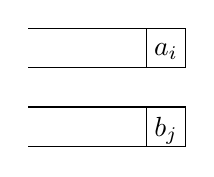
\begin{tikzpicture}[every node/.style={circle,inner sep=0pt}]
				\draw (0,1) -- (2,1) -- (2,1.5) -- (0,1.5);
				\draw (1.5,1) -- (1.5,1.5);
				\draw (1.75,1.2) node {\(a_{i}\)};
				\draw (0,0) -- (2,0) -- (2,.5) -- (0,.5);
				\draw (1.5,0) -- (1.5,.5);
				\draw (1.75,.2) node {\(b_{j}\)};
			\end{tikzpicture}
		\end{center}
		
		\(a_{i} = b_{j} \rightarrow\) Bewertung \(d(i-1,j-1)\)
	\item Missmatch
		\begin{center}
			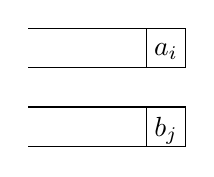
\begin{tikzpicture}[every node/.style={circle,inner sep=0pt}]
				\draw (0,1) -- (2,1) -- (2,1.5) -- (0,1.5);
				\draw (1.5,1) -- (1.5,1.5);
				\draw (1.75,1.2) node {\(a_{i}\)};
				\draw (0,0) -- (2,0) -- (2,.5) -- (0,.5);
				\draw (1.5,0) -- (1.5,.5);
				\draw (1.75,.2) node {\(b_{j}\)};
			\end{tikzpicture}
		\end{center}
		
		\(a_{i} \neq b_{j} \rightarrow\) Bewertung \(d(i-1,j-1)+1\)
	\item Löschen / Hinzufügen
		\begin{center}
			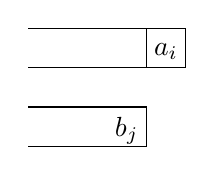
\begin{tikzpicture}[every node/.style={circle,inner sep=0pt}]
				\draw (0,1) -- (2,1) -- (2,1.5) -- (0,1.5);
				\draw (1.5,1) -- (1.5,1.5);
				\draw (1.75,1.2) node {\(a_{i}\)};
				\draw (0,0) -- (1.5,0) -- (1.5,.5) -- (0,.5);
				\draw (1.25,.2) node {\(b_{j}\)};
			\end{tikzpicture}
		\end{center}
		
		Bewertung \(d(i-1,j)+1\)
		\begin{center}
			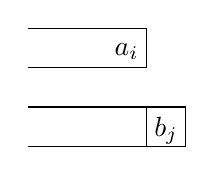
\begin{tikzpicture}[every node/.style={circle,inner sep=0pt}]
				\draw (0,1) -- (1.5,1) -- (1.5,1.5) -- (0,1.5);
				\draw (1.25,1.2) node {\(a_{i}\)};
				\draw (0,0) -- (2,0) -- (2,.5) -- (0,.5);
				\draw (1.5,0) -- (1.5,.5);
				\draw (1.75,.2) node {\(b_{j}\)};
			\end{tikzpicture}
		\end{center}
		
		Bewertung \(d(i,j-1)+1\)
\end{itemize}
Man wählt in jeden Schritt die Möglichkeit mit der besten Bewertung
\begin{equation*}
d(i,j) = \left\{
	\begin{array}{l l}
		j & \quad \text{für } i=0\\
		i & \quad \text{für } j=0\\
		\begin{array}{l l}
			\min \{&d(i-1,j-1) + 1_{a_{i} \neq b_{j}},\\
			&d(i-1,j) + 1,\\
			&d(i,j-1) + 1 \}
		\end{array} & \quad \text{für } i,j >0
  \end{array} \right.
\end{equation*}
wobei gilt:
\begin{equation*}
	  1_{a_{i} \neq b_{j}} = \left\{
	\begin{array}{l l}
		0 & \text{für } x = y \\
		1 & \text{für } x \neq y
	\end{array}
	\right.
\end{equation*}
Der Aufwand für die Berechnung in einem 2-dimensionalten Feld beträgt:
\begin{equation*}
	\underbrace{\mathcal{O}(n \cdot m)}_{\textrm{Größe der Tabelle}} \cdot \underbrace{\mathcal{O}(1)}_{\textrm{Vergleichsoperation}}
\end{equation*}
mit \(n = |a|, m= |b|\)

\subsubsection{Beispiel\protect\footnote{\url{https://youtu.be/qp8YwtvS3Uo}}}
Berechen Sie die Edierdistanz der Wörter: APFEL, PFERD.
\begin{center}
	\begin{tabular}{c|cccccc}
		& \(\varepsilon\) & A & P & F & E & L \\ \hline
	\(\varepsilon\)		& 0 & 1 & 2 & 3 & 4 & 5 \\
	P	& 1 & 1 & 1 & 2 & 3 & 4 \\
	F	& 2 & 2 & 2 & 1 & 2 & 3 \\
	E	& 3 & 3 & 3 & 2 & 1 & 2 \\
	R	& 4 & 4 & 4 & 3 & 2 & 2 \\
	D	& 5 & 5 & 5 & 4 & 3 & \textbf{\textcolor{red}{3}}
	\end{tabular}
\end{center}

\section{Längste gemeinsame Teilffolge}
Eine längste gemeinsame Teilffolge kann durch Streichen von Zeichen erzeugt werden.
Bespiel:
\begin{figure}[htbp]
	\begin{center}
		\begin{tikzpicture}
			\node (1) {A};
			\node (2) [right of=1] {N};
			\node (3) [right of=2] {A};
			\node (4) [right of=3] {N};
			\node[cross] (5) [right of=4] {A};
			\node[cross] (6) [right of=5] {S};
			\node (8) [below of=1] {A};
			\node (9) [below of=2] {N};
			\node (10) [below of=3] {A};
			\node (11) [below of=4] {N};
			\node[cross] (12) [below of=5] {E};
			\node[cross] (13) [left of=8] {B};
		\end{tikzpicture}
	\end{center}
\end{figure}
Die längste gemeinsame Teilffolge ist in diesem Bespiel 4.


Sei \(d(i,j)\) die Länge der längsten gemeinsamen Teilffolge von \(a_{1} \ldots a_{i}, b_{1} \ldots b_{j}\).
So gibt es folgende Möglichkeiten:

\begin{itemize}
	\item Teilffolge verlängern (sodass die letzten beiden Zeichen übereinstimmen)
		\begin{center}
			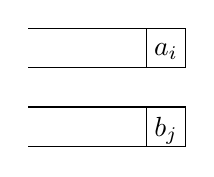
\begin{tikzpicture}[every node/.style={circle,inner sep=0pt}]
				\draw (0,1) -- (2,1) -- (2,1.5) -- (0,1.5);
				\draw (1.5,1) -- (1.5,1.5);
				\draw (1.75,1.2) node {\(a_{i}\)};
				\draw (0,0) -- (2,0) -- (2,.5) -- (0,.5);
				\draw (1.5,0) -- (1.5,.5);
				\draw (1.75,.2) node {\(b_{j}\)};
			\end{tikzpicture}
		\end{center}
		
		\(a_{i} = b_{j} \rightarrow\) Bewertung: \(d(i-1,j-1)+1\)
	\item Zeichen streichen
		\begin{center}
			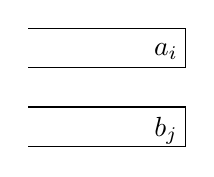
\begin{tikzpicture}[every node/.style={circle,inner sep=0pt}]
				\draw (0,1) -- (2,1) -- (2,1.5) -- (0,1.5);
				\draw (1.75,1.2) node {\(a_{i}\)};
				\draw (0,0) -- (2,0) -- (2,.5) -- (0,.5);
				\draw (1.75,.2) node {\(b_{j}\)};
			\end{tikzpicture}
		\end{center}
		\(a_{i} \neq b_{j} \rightarrow\) Bewertung: \(d(i-1,j-1)\)
	\newpage
	\item Eines der letzten beiden Zeichen streichen
		\begin{center}
			\begin{tikzpicture}[every node/.style={circle,inner sep=0pt}]
				\draw (0,1) -- (2,1) -- (2,1.5) -- (0,1.5);
				\draw (1.5,1) -- (1.5,1.5);
				\draw (1.75,1.2) node[cross] {\(a_{i}\)};
				\draw (0,0) -- (1.5,0) -- (1.5,.5) -- (0,.5);
				\draw (1,0) -- (1,.5);
				\draw (1.25,.2) node {\(b_{j}\)};
			\end{tikzpicture}
		\end{center}
		Bewertung: \(d(i-1,j)\),\\ entsprechend andere Fall: \(d(i,j-1)\)
\end{itemize}
Damit gilt:
\begin{equation*}
d(i,j) = \left\{
	\begin{array}{l l}
		0 & \quad \text{für } i=0 \text{ oder } j=0\\
		\begin{array}{l l}
			\max \{&d(i-1,j-1) + 1_{a_{i} = b_{j}},\\
			&d(i-1,j),\\
			&d(i,j-1) \}
		\end{array} & \quad \text{für } i,j >0
  \end{array} \right.
\end{equation*}
Für die Laufzeit beträgt wie bei der Edierdistanz: \(\mathcal{O}(n \cdot m) \cdot \mathcal{O}(1) = \mathcal{O}(mn)\)

\subsubsection{Beispiel}
Berechen Sie die längste gemeinsame Teilfolge  der Wörter: BANANE, ANANAS.
\begin{center}
	\begin{tabular}{c|ccccccc}
		& \ & B & A & N & A & N & E \\ \hline
		& 0 & 0 & 0 & 0 & 0 & 0 & 0 \\
	A	& 0 & 0 & 1 & 1 & 1 & 1 & 1 \\
	N	& 0 & 0 & 1 & 2 & 2 & 2 & 2 \\
	A	& 0 & 0 & 1 & 2 & 3 & 3 & 3 \\
	N	& 0 & 0 & 1 & 2 & 3 & 4 & 4 \\
	A	& 0 & 0 & 1 & 2 & 3 & 4 & 4 \\
	S	& 0 & 0 & 1 & 2 & 3 & 4 & \textbf{\textcolor{red}{4}}
	\end{tabular}
\end{center}

\section{Komplexitätsklassen}
Eine Komplexitätsklasse bezeichnet eine Menge von Problemen, welche sich in einem ressourcenbeschränkten Berechnungsmodell berechnen lassen.
Definiert wird eine Komplexitätsklasse durch eine obere Schranke für den Bedarf einer bestimmten Ressource unter Voraussetzung eines Berechnungsmodells.
Die am häufigsten betrachteten Ressourcen sind die Anzahl der notwendigen Berechnungsschritte zur Lösung eines Problems oder der Bedarf an Speicherplatz.

Folgende Beispiele sollen die Einteilung verdeutlichen:
\begin{itemize}
	\item Rasenmähen hat mindestens lineare Komplexität (in der Fläche), denn man muss die gesamte Fläche mindestens einmal überfahren.
	\item Suchen im Telefonbuch hat hingegen nur logarithmische Komplexität, denn bei einem doppelt so dickem Telefonbuch schlägt man dieses nur einmal öfter auf (siehe Kapitel \ref{sec:binaereSuche})
\end{itemize}
Nachfolgend betrachten wir die die beiden Komplexitätsklassen P und NP genauer.

\begin{description}
	\item[P] enthält alle Probleme, die sich in der Zeit \(\mathcal{O}(n^{k})\) für ein \(k>0\) entscheiden lassen (polynomialer Zeit).
		Diese sind meist effizent lösbar.
		Beispiele:
			\begin{itemize}
				\item Sortieren (\(\mathcal{O}(n \log n)\)
				\item Editierdistanz (\(\mathcal{O}(m \cdot n) \subseteq \mathcal{O}((m+n)^{2})\)
			\end{itemize}
	\item[NP] enthält alle Probleme, die sich in der Zeit \(\mathcal{O}(n^{k})\) verifizieren (Prüfen einer gültigen Belegung) lassen.
		Diese sind nur exponentieller Zeit lösbar.
		Eine Unterklasse davon sind die NP-vollständigen Probleme.
		Diese sind mindestens so schwer wie alle Probleme in NP.
		Wichtige NP-vollständige Probleme:
		\begin{itemize}
			\item Erfüllbarkeitsproblem der Aussagenlogik (Gegeben sei eine Formel der Aussagenlogik. Ist diese erfüllbar?)
			\item Hamilton-Kreis (besitzt ein Graph einen Kreis, der jeden Knoten genau einmal besucht?)
			\item Travelling Salesmann Problem
			\item Rucksack-Problem
		\end{itemize}
\end{description}
Es gilt: Wenn ein NP-vollständiges Problem in P liegt, dann liegen alle NP-voll"-stän"-di"-gen Probleme in P.
Da bisher kein derartiges Problem gefunden wurde folgt daraus: Für kein NP-vollständiges Problem ist ein polynomialer Algorithmus bekannt.


\section{Travelling Salesmann Problem}
\label{sec:TSP}
Gesucht ist die kürzeste Rundreise durch \(n\) Städte, wobei jede Stadt genau einmal besucht wird.
Das TSP ist NP-vollständig.

Sei \((d_{ij})_{1 \leq i, j \leq n}\) die entsprechende Entfernungsmatrix.
Wir betrachten den allgemeinen Fall in dem \(d_{ij} \neq d_{ji}\) sowie \(d_{ij} = \infty\) gelten kann.
Der naive Algorithmus prüft alle \(n!\) Kombinationen und hat eine Laufzeit in \(\Omega(n!) \cdot \mathcal{O}(n) = \Omega(n!)\).

Optimalitätsprinzip: Wenn eine optimale Rundreise bei Stadt 1 beginnt und dann durch k führt, dann muss der Weg von k durch die Städte in \(\{2, \ldots, n\} - \{k\}\) ebenfalls optimal sein.
Sei \(l(i,S)\) die Länge des kürzesten Pfades, der bei \(i\) beginnt, dann durch jedes \(j \in S\) genau einmal führt und bei \(n\) endet.
\begin{figure}[tbp]
	\centering
	\begin{tikzpicture}[node distance=2cm]
		\draw (0,0) circle[radius=2pt] node[align=center, below] {i};
		\draw (2,0) circle[radius=2pt] node[align=center, below] {n};
		\draw[thick,decorate,decoration={brace,amplitude=12pt}] (2,-.5) -- (0,-.5) node[midway,below, yshift=-12pt]{s};
		\draw [zigzag] (.1,0) -- (1.9,0);
		\draw (4,0) circle[radius=2pt] node[align=center, below] {i};
		\draw (5,0) circle[radius=2pt] node[align=center, below] {j};
		\draw (7,0) circle[radius=2pt] node[align=center, below] {n};
		\draw[->] (4.1,0) -- (4.9,0) node[midway,below, yshift=-12pt]{\(d_{ij}\)};
		\draw [zigzag] (5.1,0) -- (6.9,0);
		\draw[thick,decorate,decoration={brace,amplitude=12pt}] (7,-.5) -- (5,-.5) node[midway,below, yshift=-12pt]{\(S-\{j\}\)};
	\end{tikzpicture}
	\caption{Veranschaulichung Optimalitätsprinzip}
\end{figure}
Die Länge des kürzesten Rundweges ist dann \(l(n, \{1, \ldots, n-1\})\).
Es gilt:
\begin{equation*}
l(i, S) = \left\{
	\begin{array}{l l}
		d_{in} & \quad \text{für } S = \varnothing \text{(keine Zwischenstädte)}\\
		\min\limits_{j \in S} \{d_{ij} + l(S-\{j\},j)\} & \quad \text{für alle } S \neq \varnothing
  \end{array} \right.
\end{equation*}

Mit Hilfe dieses Algorithmuses kann eine Matix erstellt werden, in welcher die Länge der Rundwege gepeichert werden.
In der x-Achse werden die Knoten von 1 bis \(n-1\) eingetragen und in der y-Achse die Teilmengen in aufsteigender Mächtigkeit.
Dieser besitzt eine Laufzweit von \(\mathcal{O}(2^{n-1} \cdot (n-1)) \cdot \mathcal{O}(n) = \mathcal{O}(n^{2} \cdot 2^{n})\).
Diese wächst langsamer als \(\mathcal{O}(n!)\).

Gegeben sei der nachfolgende Graph mit 4 Städten.
Gesucht ist der kürzeste Weg zur Stadt 4.
\begin{figure}[htbp]
	\begin{center}
		\begin{tikzpicture}[node distance=1.8cm]
			\node[state] (1) {1};
			\node[state] (2) [right of=1] {2};
			\node[state] (3) [below of=2] {3};
			\node[state] (4) [below of=1] {4};
			\path[-]
				(1) edge node[above] {2} (2)
					edge node[left, above] {1} (3)
					edge node[left] {2} (4)
				(2) edge node[right] {2} (3)
					edge node[right, below] {1} (4)
				(3) edge node[below] {2} (4);
		\end{tikzpicture}
	\end{center}
\end{figure}
\begin{center}
	\begin{tabular}{c|cccc}
	\{1,2,3\}	& X & X & X & Lösung: \begin{tabular}[x]{@{}c@{}c@{}}\(2+4=6\)\\\(1+5=6\)\\\(2+4=6\)\end{tabular}  \\ 
	\{2,3\}	& \begin{tabular}[x]{@{}c@{}}\(1+3=4\)\\\(2+4=6\)\end{tabular} & X & X & \\
	\{1,3\}	& X & \begin{tabular}[x]{@{}c@{}}\(2+3=5\)\\\(2+3=5\)\end{tabular} & X & \\
	\{1,2\}	& X & X & \begin{tabular}[x]{@{}c@{}}\(2+4=6\)\\\(1+3=4\)\end{tabular} & \\
	\{3\}	& \(2+2=3\) & \(2+2=4\) & X 		& \\
	\{2\}	& \(2+1=3\) & X 		& \(2+1=3\) & \\
	\{1\}	& X			& \(2+2=4\) & \(1+2=3\) & \\
	\{\(\varnothing\)\}		& 2 & 1 & 2 & \\ \hline
			& 1 & 2 & 3 & 4 
	\end{tabular}
\end{center}

\begin{shaded}
  \noindent
  \textbf{Def.:} Sei \(\varepsilon > 1\).
	Ein Minimierungsproblem heißt \(\varepsilon\)-approximierbar, wenn es einen Algorithmus mit polynomieller Laufzeit gibt, der eine Lösung liefert, die höchstems um \(\varepsilon\) größer ist als das Optimum.
\end{shaded}
Für \(P \neq NP\) ist das TSP für kein \(\varepsilon > 1\) approximierbar.
Falls die Entfernungsmatrix jedoch die Dreiecksungleichung \[d_{uv} \leq d_{uw} + d_{wv}\] gilt (\(\Delta\)-TSP), dann ist das Problem \(\frac{3}{2}\)-approximierbar.
Die Gültigkeit der Dreiecksungleichung lässt sich immer erreichen indem ggf. Kanten durch kürzere Wege ersetzt werden.

Ein Spezialfall des \(\Delta\)-TSP ist das Euklidischen TSP, bei dem die Abstände gleich dem geometrischen Abstand sind. Für jedes \(\delta > 1\) ist das Euklidische TSP in der Ebene \(1+\frac{1}{\delta}\)-approximierbar.
Der zugehörige Approximationsalgorithmus besitzt eine Laufzeit in \(\mathcal{O}(n \log(n))^{\mathcal{O}(\delta)}\).

Anwendungen des TSP:
\begin{itemize}
	\item Roboter soll Löcher in eine Platine bohren
	\item Auf einer Fertigungsstraße sollen Produkte \(P_{1}, \ldots, P_{n}\) herrgestellt werden.
		Dabei muss die Fertigungsstraße jeweils umgerüstet werden.
		Wenn \(d_{uv}\) die Zeit ist, die für das umrüsten von \(P_{U}\) nach \(P_{V}\) benötigt wird, muss ein TSP für (\(d_{uv}\)) gelöst werden..
		Für kleine \(n\) kann das exakte TSP und sonst das \(\Delta\)-TSP (Bedingung: Dreiecksungleichung)zur Approximation des Optimums verwendet werden.
	\item DNA-Sequenzierung (Erzeugung von DNA-Bruchstücken, Suche nach Über\-lap\-pungen, kürzester Pfad durch diese Knoten (Besser wäre allerdings der Aufbau einen Graphen und Suche eines euklidischen Kreises))
\end{itemize}



\section{Rucksackproblem}
Das Rucksackproblem ist ein Optimierungsproblem der Kombinatorik.
Aus einer Menge von Objekten, die jeweils ein Gewicht und einen Nutzwert haben, soll eine Teilmenge ausgewählt werden, deren Gesamtgewicht eine vorgegebene Gewichtsschranke nicht überschreitet.
Unter dieser Bedingung soll der Nutzwert der ausgewählten Objekte maximiert werden.
Anwendungen:
\begin{itemize}
	\item öffentliche Haushaltsführung
	\item Reduzierung des Verschnitts (Bsp. Fließen, Folien)
	\item Logistik (Bsp. Transport mittels Frachschiff)
\end{itemize}

Gegebenen seien n Gegenstände mit den Werten \(x_{1}, \dots, x_{n}\).
Gesucht ist eine Auswahl, die den Wert der Gegenstände maximiert und einen Schwellwert \(y\) nicht überschreitet.

Das Rucksackproblem ist NP-vollständig, es lässt sich mit einem dynamischen Pro\-gram\-mier-Algorithmus wie folgt lösen:
Sei \(r(n,y)\) der Wert einer Lösung des Rucksackproblems für die Werte \(x_{1}, \dots, x_{n}\) und der Rucksackgröße \(y\) dann gilt:
 \[r(n,y) = \left\{
			\begin{array}{l l}
				0 				& \quad \text{für } n=0\\
				r(n-1,y) 		& \quad \text{für } n>0 \wedge x_{n} > y \\
				\begin{array}{l l}
					\max \{
						r(n-1,y),\\
						r(n-1,y-x_{n})+x_{n}
					\}
				\end{array} & \quad \text{sonst}
		\end{array} \right.\]

Die Laufzeit des Rucksack-Algorithmuses beträgt: \(\mathcal{O}(ny)\).
Es stellt sich daher die Frage ob dies ein polynomieller Algorithmus für das Rucksackproblem ist (woraus P=NP folgen würde)?

Probleme werden in der Komplexitätstheorie als Mengen dargestellt und die Laufzeit als Funktion in der Länge einer Instanz.
Die Länge einer Instanz ist \((x_1, \dots, x_n, y)\).
Um \(y\) über dem Alphabet \({0,1}\) (binär) darzustellen werden \(\log_2y + \mathcal{O}(1)\) Zeichen benötigt.
Als Funktion der Länge der Eingabe ergibt sich für die Laufzeit \(ny = n2^{\log_2y}\).
Die Laufzeit ist damit exponentiell in der Länge der Eingabe.

\begin{shaded}
	\noindent
	\textbf{Def.:} Ein Algorithmus heißt pseudopolynomiell, wenn seine Laufzeit durch ein Polynom in der Eingabelänge und der größten, in der Eingabe vorkomenden Zahl beschränkt ist.
\end{shaded}
Das Rucksackproblem ist pseudopolynomiell: Sein \(|w|\) die Eingabelänge und \(m = \max(x_1, \dots, x_n, y)\) (Das Längste Wort der Kodierung).
Dann gilt: \(n\leq |w|\), woraus \(\mathcal{O}(ny) \subseteq \mathcal{O}(|w|m)\) folgt.